\documentclass[10pt,aspectratio=169,dvipsnames]{beamer} % sets document type, default font size, slide aspect ratio, and loads color names
\usetheme[color/block=transparent]{metropolis} % sets the theme of the document

\usepackage[absolute,overlay]{textpos} % allows absolute positioning of text
\usepackage{booktabs} % enhances quality of tables
\usepackage[utf8]{inputenc} % allows input encoding in UTF-8
\usepackage{tikz} % used for creating vector graphics
\usetikzlibrary{arrows.meta} % loads additional arrow types
\usepackage[europeanresistors,americaninductors]{circuitikz} % for drawing electrical circuits
\usepackage[scale=2]{ccicons} % loads Creative Commons icons
\usepackage[official]{eurosym} % loads the official symbol for the Euro
\usepackage{hyperref} % allows creating hyperlinks in the document

\newcommand{\ra}[1]{\renewcommand{\arraystretch}{#1}} % creates command to adjust spacing between rows
\newcommand{\hrefc}[2]{\href{#1}{\bf\color{blue}{\underline{#2}}}} % defines command for underlined, blue hyperlink
\newcommand{\urlc}[1]{\hrefc{#1}{#1}} % defines command for URL hyperlink

\newcommand{\R}{\mathbb{R}} % creates a shortcut for typing real numbers symbol
\newcommand{\ubar}[1]{\text{\b{$#1$}}} % defines a command for underlined text

\xdefinecolor{TUred}{RGB}{197,14,31} % defines a new color TUred
\setbeamerfont{alerted text}{series=\bfseries} % sets the font of alerted text to bold
\setbeamercolor{alerted text}{fg=TUred} % sets the color of alerted text to TUred
\setbeamercolor{background canvas}{bg=white} % sets the background color to white
\setbeamercolor{frametitle}{bg=lightgray!40, fg=TUred} % sets the background color of the frame title to light gray and text color to TUred
\setbeamercolor{title}{fg=TUred} % sets the color of the title to TUred

\addtobeamertemplate{frametitle}{}{% adds image to every frame title
  \begin{textblock*}{100mm}(1.01\textwidth,2pt)
    
\includegraphics[width=1.5cm]{images/TUB.png}
    \end{textblock*}}

\def\l{\lambda} % defines a shortcut for lambda symbol
\def\m{\mu} % defines a shortcut for mu symbol
\def\d{\partial} % defines a shortcut for partial symbol
\def\cL{\mathcal{L}} % defines a shortcut for caligraphic L symbol
\def\co{CO${}_2$} % defines a shortcut for CO2 symbol
\def\el{${}_{el}$} % defines a subscript for el
\def\th{${}_{th}$} % defines a subscript for th
\def\gas{${}_{gas}$} % defines a subscript for gas

\setbeamercolor{framesource}{fg=gray} % sets color of framesource to gray
\setbeamerfont{framesource}{size=\tiny} % sets font size of framesource to tiny
\newcommand{\source}[1]{% creates command for inserting a source footnote
\begin{textblock*}{5cm}(10.5cm,8.35cm)
    \begin{beamercolorbox}[ht=0.5cm,right]{framesource}
        \usebeamerfont{framesource}\usebeamercolor[fg]{framesource} {#1}
    \end{beamercolorbox}
\end{textblock*}}

\graphicspath{{../results/}} % sets the path where graphics can be found
\DeclareGraphicsExtensions{.pdf,.jpeg,.png,.jpg} % defines the types of graphic files that can be used

\def\goat#1{{\scriptsize\color{green}{[#1]}}} % defines a command for green, scriptsize text

\let\olditem\item % saves the old item command
\renewcommand{\item}{\olditem\vspace{5pt}} % redefines the item command to add space after each item


\title{System-level impacts of 24/7 carbon-free electricity procurement in Europe}

%\subtitle{---}
\author{
  Iegor Riepin, Tom Brown\\
  \hrefc{https://tub-ensys.github.io/}{Department of Digital Transformation in Energy Systems}, TU Berlin
}

\date{12 October 2022}

\titlegraphic{%
  \vspace{0cm}
  \hspace{10.7cm}
    
\includegraphics[trim=0 0cm 0 0cm,height=1.2cm,clip=true]{images/TUB.png}

\vspace{5.1cm}
   
}

\begin{document}

\maketitle


\begin{frame}
  \frametitle{Acknowledgements}

  \begin{itemize}
    \item {\bf Funding:} This study was supported by a grant from Google, Inc. 
    \item {\bf Acknowledgements:} The authors acknowledge members of the Google energy markets and policy team 
    for their feedback and inputs on earlier drafts of this report. 
    Also, warm regards to the \hrefc{https://pypsa.org/}{PyPSA team} and many contributors to the open-source 
    PyPSA energy system modelling tool used in this study (see: \hrefc{https://github.com/PyPSA/PyPSA}{github.com/PyPSA})
    \item 
    {\bf Copyright} Unless otherwise stated, graphics and text are Copyright \copyright Tom Brown and Iegor Riepin, 2022.
    Graphics and text for which no other attribution are given are licensed under a 
    \href{https://creativecommons.org/licenses/by/4.0/}{CC BY 4.0}.  {\footnotesize \ccby} 
    \item The content of this study, including any errors or omissions are the responsibility
    of the authors alone.
  \end{itemize}

\end{frame}


\begin{frame}

  \frametitle{Table of Contents}
  \setbeamertemplate{section in toc}[sections numbered]
  \tableofcontents[hideallsubsections]
\end{frame}


%----------------------------------------
%----------------------------------------

\section{Introduction}


\begin{frame}{Introduction}

  \centering
    \begin{itemize}
    \item Climate change is driving a global effort to rapidly decarbonise 
    electricity systems across the globe. 
    Many public and private energy buyers have joined this effort and highlight
    their sustainable credentials by procuring renewable energy with the 
    Power Purchase Agreements (PPAs).
    \item Such \alert{voluntary commitments accelerate the deployment of renewable 
    capacity} above the policy requirements in the countries and jurisdictions
    these companies operate. This facilitates faster
    transformation of electricity markets by driving renewables
    techologies down the experience curves.
    \item Additionally, many early actors in the field helped pave the way for followers 
    \hrefc{https://www.gstatic.com/gumdrop/sustainability/247-carbon-free-energy.pdf}{by 
    developing methods and establishing standard contracts} for clean energy procurement.
    \end{itemize}
  
\end{frame}



\begin{frame}{Introduction}

  \begin{columns}[T]
    \begin{column}{6cm}
      \begin{itemize}
        \item   PPAs typically allow for renewable energy to match supply and
        demand on average over a long period of time. 
        \item For example, more than 370 members of the \href{https://www.there100.org/}{RE100} group have committed to purchasing enough renewable energy to match
        \alert{100\% of their electricity consumption on an annual basis}.
      \end{itemize}
    \end{column}

  \begin{column}{10cm}
      \centering
      
      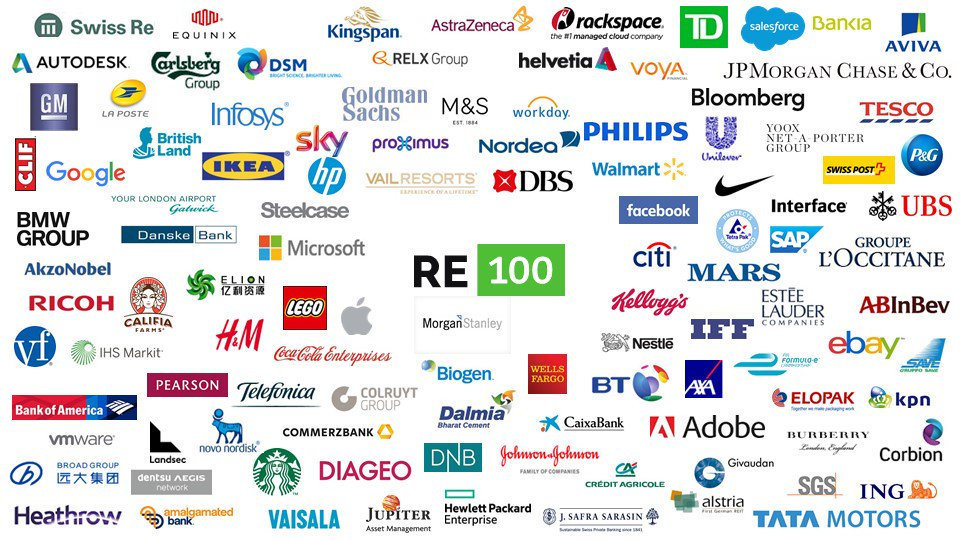
\includegraphics[width=10cm]{images/100re-companies.jpg}
      \vspace{.1cm}
      {\footnotesize
      More than 370 companies have joined \hrefc{https://www.there100.org/}{RE100}
      }
    \end{column}
    \end{columns}

    \source{source: \href{https://www.there100.org/}{RE100}}
\end{frame}
  


\begin{frame}{Introduction}
  
    \begin{itemize}
    \item However, electricity buyers that commit to 100\% annual matching 
    from renewable energy sources still face times when generation 
    from wind and solar generators is not sufficient to match 
    the companies’ electricity demand. 
    \item Thus, although buyers match their demand on a \alert{yearly} basis with 
    renewable energy, on an \alert{hourly} basis they still have hours 
    when they have to rely on carbon-emitting technologies available 
    on a local market, such as coal and gas-fired power plants.
    \end{itemize}

  \centering
  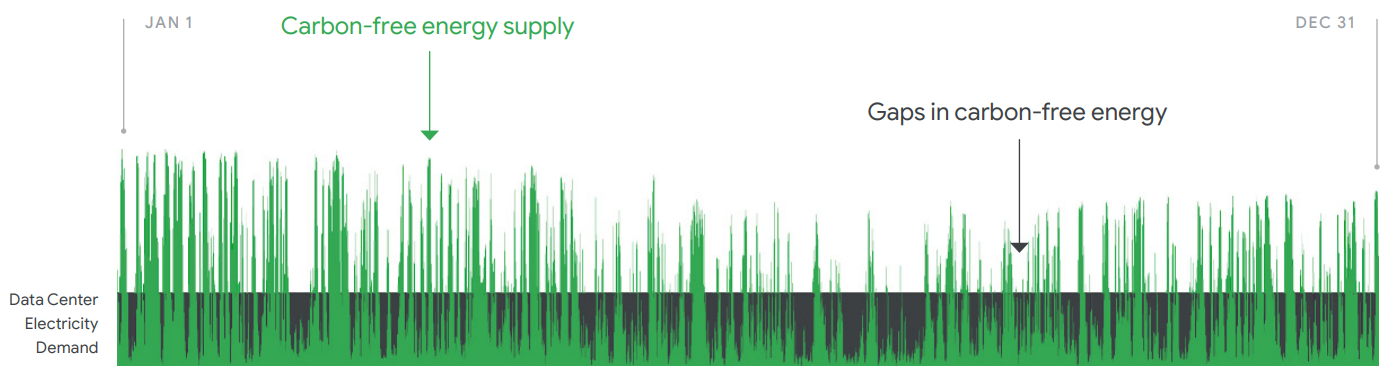
\includegraphics[width=14cm]{images/google-year.png}
  \source{\href{https://www.gstatic.com/gumdrop/sustainability/247-carbon-free-energy.pdf}{source: Google 2021, 24/7 CFE: Methodologies and Metrics}}
           
\end{frame}



\begin{frame}{Introduction}
  
  More generally, 100\% annual matching leads to many challenges 
  from the electricity buyers' and system perspectives: 
  \begin{itemize}
  \item No \alert{simultaneity} - variable generation of wind and solar power is not aligned with the 
  buyer’s electricity consumption profile.
  \item Lack of \alert{additionality} - some buyers procure unbundled guarantees of origin from existing 
  facilities, which does not lead to additional renewable generation.
  \item Displaced \alert{location} - some buyers procure  PPAs from locations far away from their consumption.
  \item Exposure to \alert{risk} - electricity buyers are exposed to price volatility 
  in local electricity markets.
  \item Need for \alert{backup} - electricity system has to maintain backup and flexibility options 
  for hours with low renewable generation.
  \end{itemize}
  
\end{frame}



\begin{frame}{24/7 carbon-free energy}

  \centering

  There is growing interest from leaders in voluntary clean
  electricity procurement to cover their consumption 
  with clean energy supply on a \alert{truly 24/7 basis}. \\
  \vspace{0.3cm}
  Achieving 24/7 Carbon-Free Energy (CFE) means that every kilowatt-hour of electricity consumption is met
  with carbon-free electricity sources, \alert{every hour of every day}.
  
\end{frame}



\begin{frame}{24/7 carbon-free energy}
  
  \begin{columns}[T]
  \begin{column}{8cm}

    \begin{itemize}
    \item The \hrefc{https://www.un.org/en/energy-compacts/page/compact-247-carbon-free-energy}{24/7 Carbon-free Energy Compact} 
    initiative was launched in 2021 by Sustainable Energy for All and the United Nations. 
    It now includes more than 80 companies, policymakers, investors, and organizations 
    on a mission to realize a 24/7 Carbon-Free Energy future. 

    \item One of the forefront runners in 24/7 initiative is Google Inc. In 2020 the company committed 
    \hrefc{https://www.gstatic.com/gumdrop/sustainability/247-carbon-free-energy.pdf}{to the goal} 
    of operating entirely on a 24/7-CFE approach at all its data centres and campuses worldwide by 2030. 
    Shortly after, Google published 
    \hrefc{https://www.gstatic.com/gumdrop/sustainability/policy-roadmap-carbon-free-energy.pdf}{a policy roadmap} 
    on achieving the 24/7-CFE goal.

    \end{itemize}
  \end{column}

  \begin{column}{8cm}
    \centering
    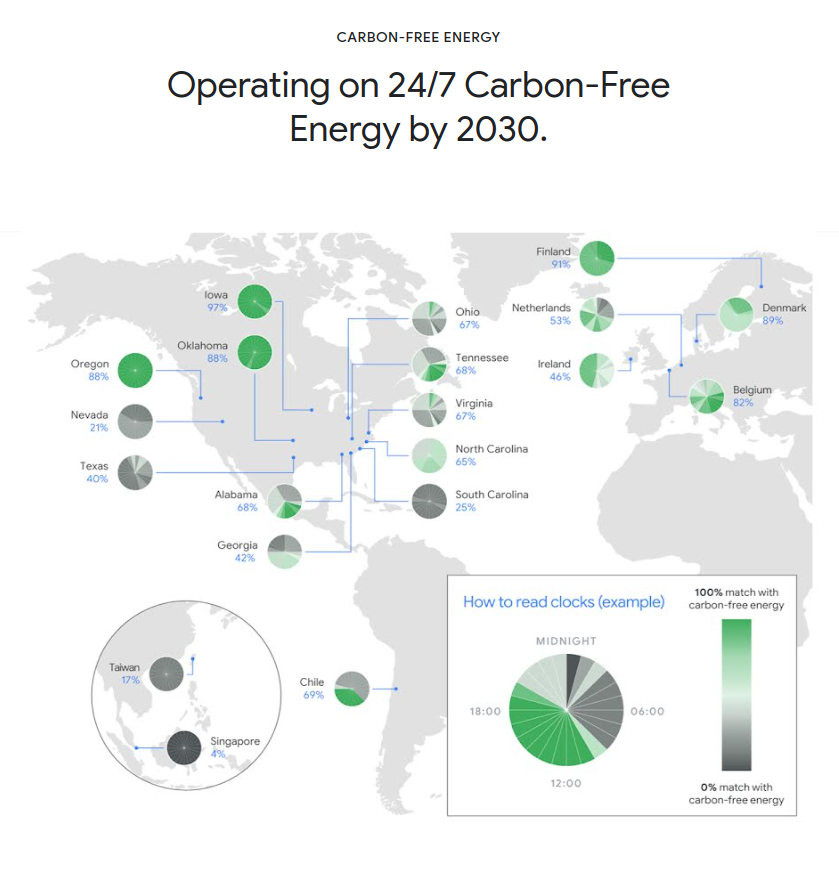
\includegraphics[width=7.5cm]{images/247-google-web.png}
    \vspace{.1cm}
  \end{column}

  \source{\href{https://sustainability.google/progress/energy/}{Google Inc.}}
  \end{columns}
  
\end{frame}



\begin{frame}{Yearly versus hourly matching}
  
  The 24/7 CFE procurement has potential benefits over the 100\% renewable matching:
  
  \begin{itemize}
  \item Ensure match of electricity consumption with carbon-free resources 
        on an \alert{hourly basis}.
  \item Enable much \alert{deeper reductions in CO$_2$} emissions assosiated 
        to buyer's electricity consumption.
  \item Ensure that contracted power is \alert{additional} (i.e. leads to new capacity).
  \item Ensure that power comes from the \alert{same bidding zone}.
  \item Enable procurement of \alert{carbon-free} rather than renewable technologies 
        (such as advanced “clean dispatchable” power generation and long-duration energy storage).
  \end{itemize}
  
\end{frame}



\begin{frame}{Focus of the study}
  
  In this study, we investigate both the \alert{means and costs of 24/7 procurement} for companies
  and the \alert{system impacts} for the rest of the European electricity system. 

  We focus our analysis on the following quesitons:

    \begin{enumerate}
    \item How can companies following 24/7~CFE procurement achieve hourly matching?
    \item What is the cost premium of 24/7~CFE versus the 100\% annual matching?
    \item To which extent can technologies, such as long-duration storage or advanced dispatchable
          clean generators, help to achieve the 24/7~CFE goal?
    \item To which extent can 24/7~CFE contribute to reductions in CO$_2$
          emissions intensity of buyer's consumption? 
    \item If many companies follow the 24/7~CFE approach, how does this effect the rest of
          the energy system?
    \end{enumerate}
  
\end{frame}



\begin{frame}{Quick summary}
  
  \begin{columns}[T]
  \begin{column}{9cm}
  \centering

    \begin{itemize}
    \item Key findings
    \end{itemize}
  \end{column}
  \end{columns}
  
\end{frame}

%----------------------------------------
%----------------------------------------

\section{Methodology and study design}


\begin{frame}
  \frametitle{PyPSA: an energy systems modelling toolbox}

\begin{columns}[T]
\begin{column}{7cm}

{\small
  \begin{itemize}
  \item PyPSA (Python for Power System Analysis) is an open source toolbox 
  for for state-of-the-art energy system modelling.
  \item Fills gap between power flow software (e.g. PowerFactory,
  MATPOWER) and energy system planning software (e.g. TIMES, OSeMOSYS).
  \item PyPSA develoment and maintenance is coordinated by the TU Berlin,
  \hrefc{https://www.ensys.tu-berlin.de/}{Department of Energy Systems}.  
  \item PyPSA is used worldwide by dozens of research institutes and companies.\\
  See \hrefc{https://pypsa.readthedocs.io/en/latest/users.html}{list of users}.
  \end{itemize}
}

\end{column}

\begin{column}{9cm}

\centering
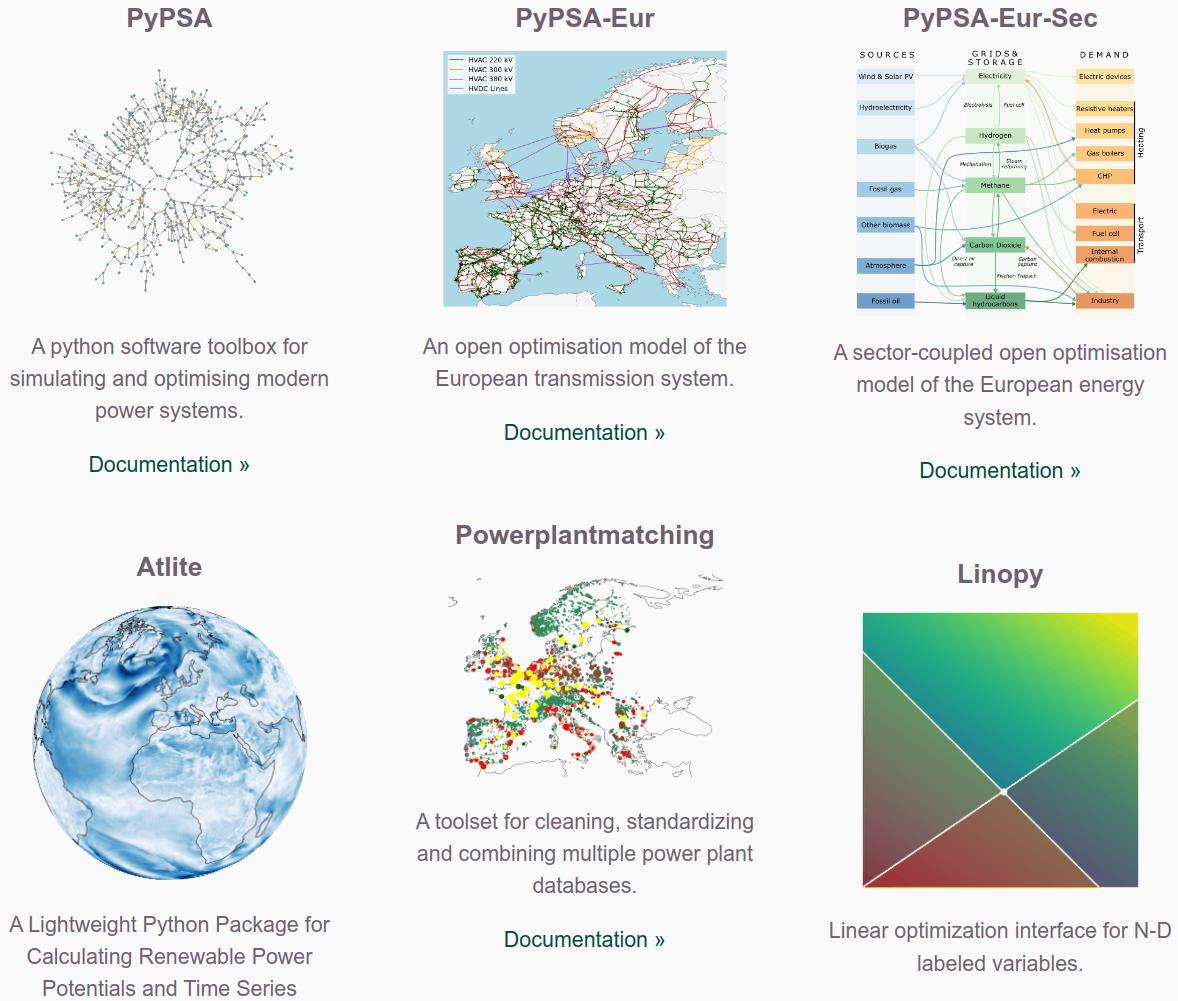
\includegraphics[width=8.5cm]{images/pypsa-web.png}
\source{\href{https://pypsa.org/}{PyPSA}}

\end{column}
\end{columns}

\end{frame}



\begin{frame}
  \frametitle{PyPSA-Eur(-Sec): open models of the European energy system}

  \begin{columns}[T]
  \begin{column}{7cm}
  {\small
  \begin{itemize}
  \item PyPSA-Eur is an open model of the European power system at the transmission network 
  level that covers the full ENTSO-E area.
  \item Only freely available and open data.
  \item Automated and configurable software pipeline from raw data to optimised electricity system.
  \item Adjustable temporal and spatial resolution.
  \item See \hrefc{https://pypsa-eur.readthedocs.io/en/latest/}{documentation}
  and \hrefc{https://docs.google.com/presentation/d/1mzj4X9uuO58gUvkhVMRCFWOJUWbs6NR9SNZe-RIkkNo/edit?usp=sharing}{feature summary} 
  for more details.
  \item PyPSA-Eur{\bf-Sec} version of the model adds building heating, transport and industry sectors, as well as gas networks.
  \end{itemize}
  }
  \end{column}

  \begin{column}{9cm}
    \centering
  {\footnotesize
    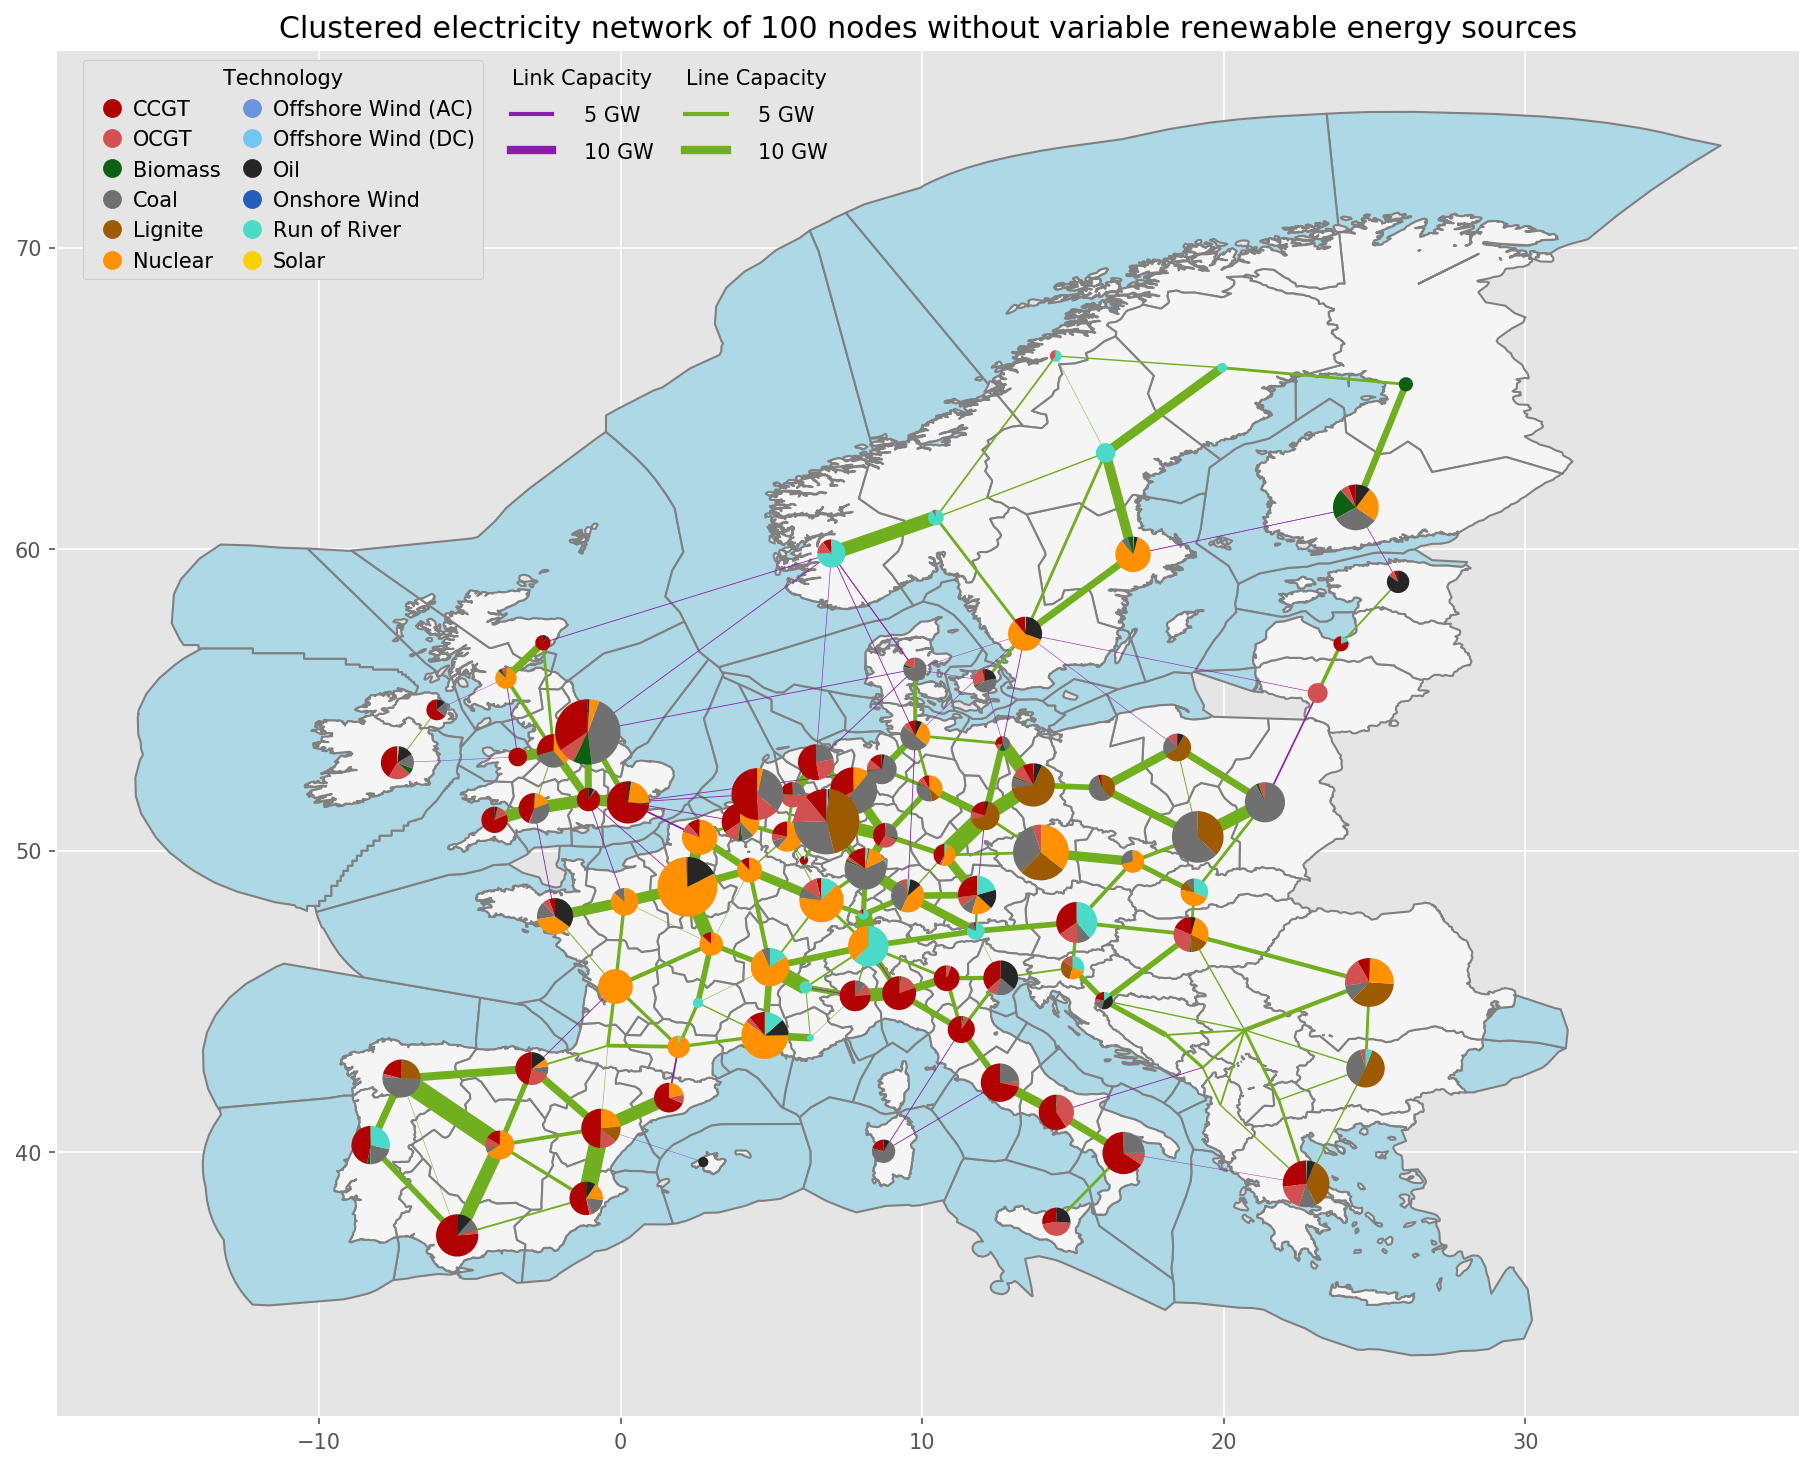
\includegraphics[width=8cm]{images/elec_s_100.png}
  
   \vspace{0.1cm}
   PyPSA-Eur(-Sec) suite of models are available on \hrefc{https://github.com/PyPSA}{GitHub}
  }
  \end{column}
  
  \end{columns}

\end{frame}



\begin{frame}{Modeling 24/7 CFE procurement}
  \begin{columns}[T]
  \begin{column}{7cm}
  {\small

  \begin{itemize}
  \item We implement a set of additional constraints to the PyPSA-Eur 
  to model a situation when a fraction of corporate and industry (C\&I) demand 
  commits to the 24/7~CFE procurement.
  \item The model optimises investment and operational decisions to meet projected
  electricity demand for the 24/7~CFE consumers, as well as
  the demand of other consumers in the European electricity system, while meeting all
  relevant engineering, reliability, and policy constraints.
  \end{itemize}
  }
  \end{column}

  \begin{column}{9cm}
  \centering
  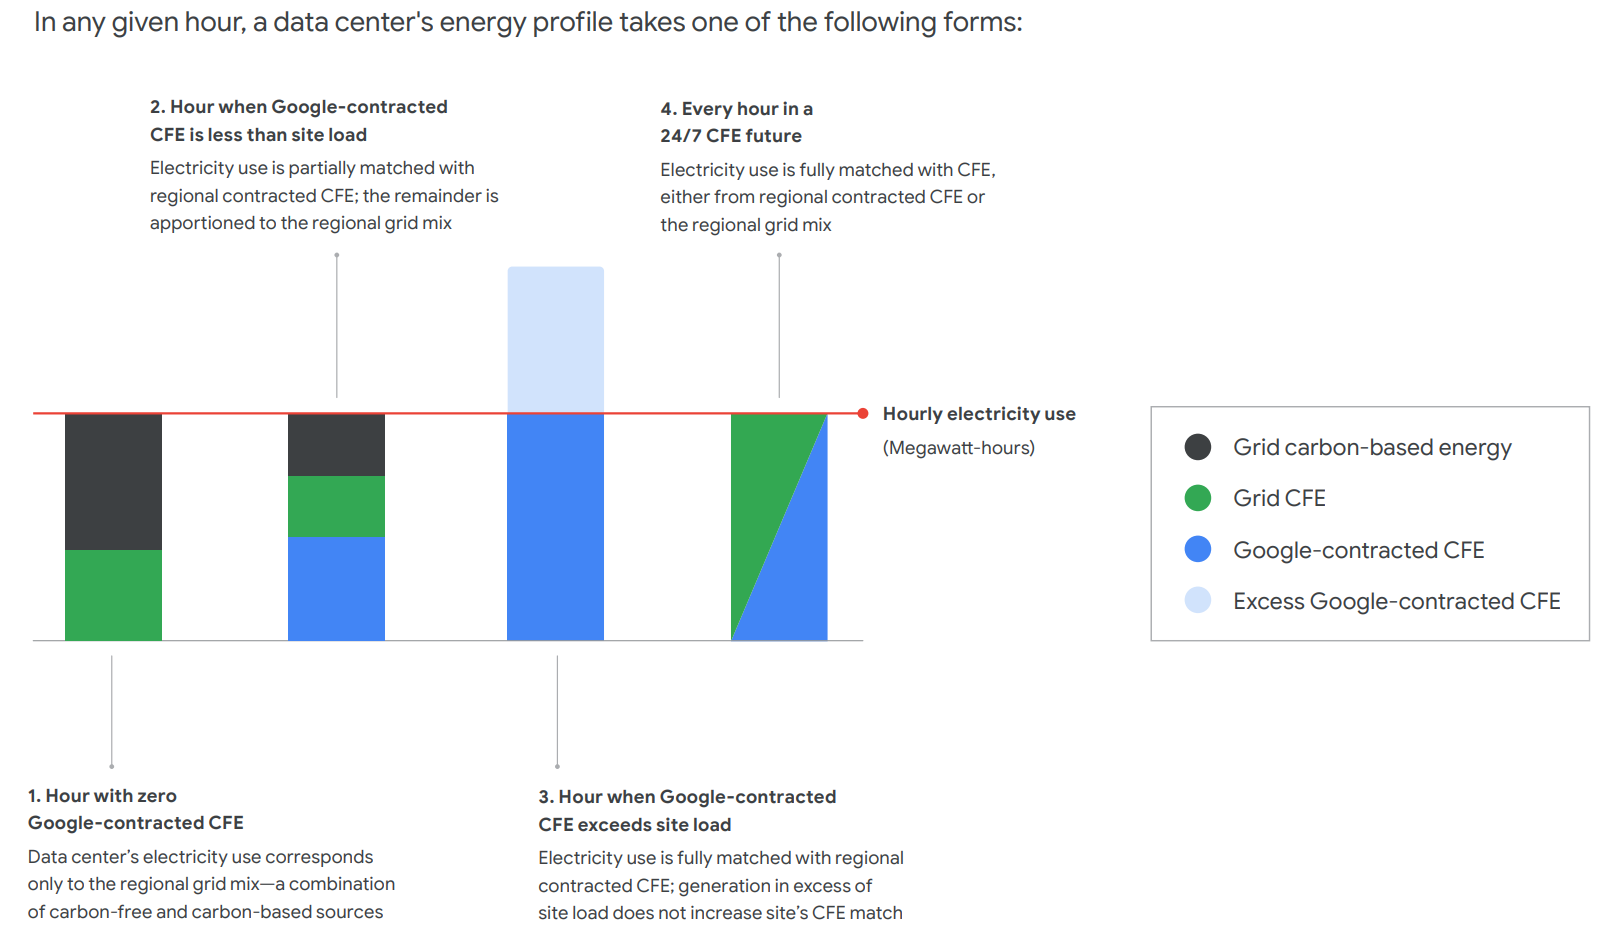
\includegraphics[width=8.5cm]{images/247-concept.png}
  {\footnotesize
  The methods are based on the Google's CFE procurement framework, presented in paper
  \hrefc{https://www.gstatic.com/gumdrop/sustainability/24x7-carbon-free-energy-methodologies-metrics.pdf}{"24/7 Carbon-Free Energy: Methodologies and Metrics"}
  }
  \source{\href{https://www.gstatic.com/gumdrop/sustainability/24x7-carbon-free-energy-methodologies-metrics.pdf}{source: Google 2021, 24/7 CFE: Methodologies and Metrics}}
  \end{column}

  \end{columns}

\end{frame}



\begin{frame}{Implementation of C\&I demand and supply}

  {\small

  The model optimizes portfolio of carbon-free generation and storage technologies 
  procured by the participating C\&I consumers. The portfolio assets have to be located 
  in the same market zone.

  The hourly demand of C\&I consumers $d_t$ for hour $t$ can be met 
  by a combination of the following: \\
    \begin{itemize}
      \item dispatch $g_{r,t}$ of procured CFE generators $r\in CFE$ 
      \item dispatch $\bar{g}_{s,t}$ of procured storage technologies $s\in STO$
            (requires charge $\ubar{g}_{s,t}$)
      \item imports from the grid $im_t$.
    \end{itemize}
    }

\begin{columns}

  \begin{column}{7cm}
  \begin{equation*}
  \sum_{r\in CFE} g_{r,t} + \sum_{s\in STO} \left(\bar{g}_{s,t} - \ubar{g}_{s,t}\right) - ex_t + im_t  =  d_t \hspace{.7cm} \forall t
  \end{equation*}

  \vspace{0.3cm}
  {\small NB: the excess from the local supply $ex_t$ can either be sold to the grid 
  at market prices or curtailed.}
  \end{column}

\begin{column}{5cm}
\centering
\begin{circuitikz}
  \draw (0,13.5) to [short,i^=$im_t$]  (1.5,13.5) to (1.5,13);
  \draw [ultra thick] (0,13) node[anchor=south]{} -- (4,13);
  \draw(2.5,13) |- +(0,0.5) to [short,i^=$ex_t$] +(1.5,0.5);
  \draw (0.5,13) -- +(0,-0.5) node[sground]{};
  \draw (2,12) node[vsourcesinshape, rotate=270](V2){}
  (V2.left) -- +(0,0.6);
  \draw (3.5,13) -- (3.5,12.4);
  \draw (3.5,12.4) to [esource] (3.5,11.7);
  \draw (0.5,11) node{$d_t$};
  \draw (2,11) node{$g_{CFE,t}$};
  \draw (3.5,11) node{$g_{STO,t}$};
\end{circuitikz}
\end{column}

\end{columns}

\end{frame}



\begin{frame}{Implementation of 100\% annual matching}

  {\small
  
The \alert{100\% annual matching} is modelled with a constraint (\ref{eqn:RES100}), which requires C\&I consumers 
to purchase enough renewable electricity to match all of their electricity consumption
on an annual basis.

\vspace{0.3cm}
More formally, the sum of all dispatch $g_{r,t}$ for RES generators $r\in RES$ over the year $t\in T$ 
is equal to the annual demand $d_t$ of C\&I consumers:
  \begin{equation}
    \sum_{r\in RES, t\in T} g_{r,t} = \sum_{t\in T} d_t
  \label{eqn:RES100}
  \end{equation}
  }
\end{frame}


\begin{frame}{Implementation of 24/7 CFE matching}

  {\small

  The \alert{24/7 CFE matching} is modelled with a constraint (\ref{eqn:CFE}), 
  which matches demand of C\&I consumers with carbon-free resources on an hourly basis. 

  More formally, the constraint states that sum over generators from procured CFE resources $r\in CFE$,
  discharge and charge from storage technologies $s\in STO$,
  as well as import from the grid $im_t$ multiplied by the grid's CFE factor $CFE_t$
  must be higher or equal than a certain CFE target $x$ multiplied with the total load:
  \vspace{0.1cm}
  \begin{equation}
  \sum_{r\in CFE, t\in T} g_{r,t} + \sum_{s\in STO, t\in T} \left(\bar{g}_{s,t} - \ubar{g}_{s,t}\right) - \sum_{t\in T} ex_t + \sum_{t\in T} CFE_t \cdot im_t \geq x \cdot \sum_{t\in T} d_t
  \label{eqn:CFE}
  \end{equation}
  \vspace{0.1cm}
  \noindent\fbox{%
    \parbox{\textwidth}{%
  The \alert{CFE Score} $x$~[\%] measures the degree to which hourly electricity consumption 
  is matched with carbon-free electricity generation within the regional grid.
  }}

  \noindent\fbox{%
    \parbox{\textwidth}{%
  Note that the grid CFE factor $CFE_t$ is affected by capacity procured by C\&I consumers. This
  introduces a nonconvex term to the optimization problem. We relax the problem by treating grid CFE factor
  as a parameter that is iteratively updated (starting with $CFE_t =0 \, \forall t$). 
  Similarly to the \hrefc{https://acee.princeton.edu/24-7/}{Xu et al. (2021)} study, we find that one forward pass (i.e. 2 iterations) yields very good convergence.
  }}
  }

\end{frame}



\begin{frame}{Implementation of 24/7 CFE matching}

  {\small

  The excess generation $ex_t$ from the procured resources representes clean electricity over
  and above demand of C\&I consumers following 24/7 approach in a particular hour. 
  The \alert{excess is not counted toward CFE score} -- 
  and thus it is substracted on the left-hand side of the eq. (\ref{eqn:CFE}).

  The excess generation can be stored and shifted to another hour where procured resources 
  generate less than the C\&I demand, sold to the regional grid at market prices or curtailed. 
  The total amount of excess generation is constrained to a certain level on an annual basis. 
  In this study, the limit is set to 20\% of annual 24/7 participating customer's demand:
  \vspace{0.1cm}
  \begin{equation}
  \sum_{t\in T} ex_t \leq ExLimit \cdot \sum_{t\in T} d_t
  \label{eqn:excess}
  \end{equation}

  \noindent\fbox{%
  \parbox{\textwidth}{%
  The constraint (\ref{eqn:excess}) facilitates \alert{additionality} -- 
  \hrefc{https://www.gstatic.com/gumdrop/sustainability/24x7-carbon-free-energy-methodologies-metrics.pdf}{one of the principles} 
  of the 24/7 CFE matching.
   From the modelling perspective, the limit on excess electricity ensures that CFE resources 
  procured by C\&I consumers are \emph{additional}, i.e. 24/7 procurement activities
  enable the deployment of clean electricity generation that is new to the grid. 
  }}
  }

\end{frame}



\begin{frame}{CFE factor of the regional grid}

  {\small

  The \alert{grid CFE factor} $CFEt$ in eq. (\ref{eqn:CFE}) defines the share of 
  carbon-free electricity  in grid imports by C\&I consumers following 24/7 approach. 
  The factor depends on the generation mix in the region where C\&I consumers are located, 
  as well as on the generation mix in other regions where from electricity is imported. 

  \begin{columns}
    \begin{column}{8cm}

  Using the notation on the right, the average cleanness 
  of the rest of the electricity system is:
  \begin{equation*}
  ImportCFE = \frac{A_t}{A_t + D_t}
  \end{equation*}

  The CFE factor of grid supply\footnote{Note 
  that generators contracted by 24/7 consumers (C) are excluded from the grid supply.} 
  for a given hour $t$ is:
  
  \begin{equation*}
  CFEt = \frac{B_t + ImportCFE * import_t}{B_t + E_t + import_t}
  \end{equation*}    

  \end{column}

  \begin{column}{5cm}
  \centering
  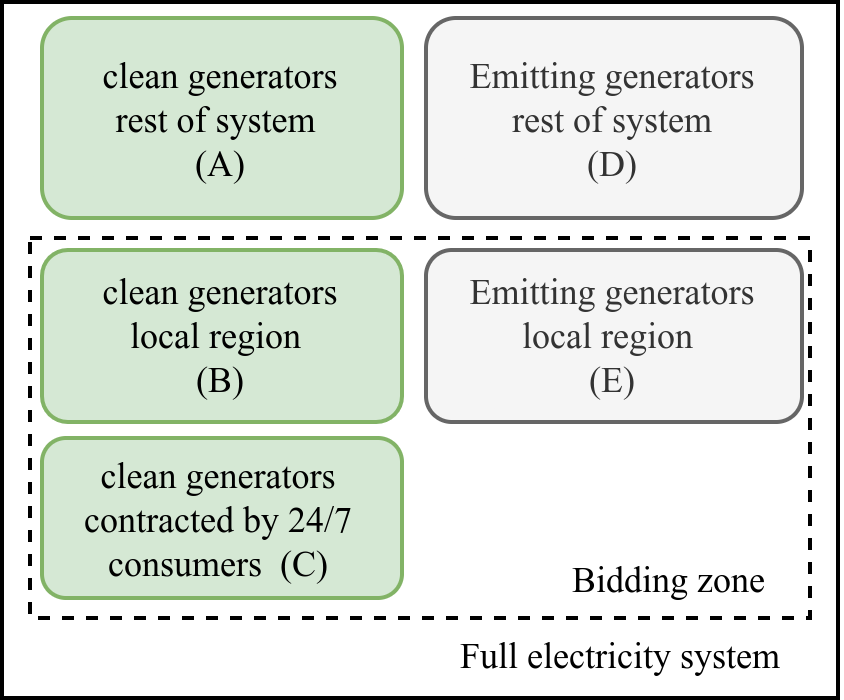
\includegraphics[width=5cm]{images/cfe.png}
  {\scriptsize
  This approach is based on \hrefc{https://acee.princeton.edu/24-7/}{Xu et al. (2021)}
  }
  \end{column}
    
  \end{columns}

  \noindent\fbox{%
  \parbox{\textwidth}{%
  CFEt can be seen as the percentage of clean electricity in each MWh of imported 
  electricity from the grid to supply participating 24/7 loads in a given hour.
  }}
  }

\end{frame}


\begin{frame}{CO$_2$ emissions rate of the regional grid and 24/7 portfolio, 1/2}

  {\small

  \alert{CO$_2$ emissions} associated with the dispatch of emitting power plants 
  in the European electricity system are part of the model solution.
  We can use this information to calculate (i) the \emph{emissionality} of generation 
  that serves participating 24/7 demand, and (ii) the \emph{avoided emissions}, i.e.,
  the difference in regional CO$_2$ emissions with and without 24/7 procurement. 
  Similarly to the logic of computing the grid CFE factor, 
  we need to consider imported emissions also in this calculation.
  
  First, let $X(D)_t$ be hourly emissions $[tCO_2]$ in the rest of the electricity system. 
  The average emissions rate of the rest of the system is calculated as:

  \begin{equation*}
  SystemEmisRate = \frac{X(D)_t}{A_t + D_t}
  \end{equation*}

  Second, let $Y(E)_t$ be hourly emissions in the regional grid where 24/7 consumers are located.
  The emissions rate of grid supply than is:

  \begin{equation*}
  GridSupplyEmisRate = \frac{Y(E)_t + SystemEmisRate * import_t}{B_t + E_t + import_t}
  \end{equation*}

  }
\end{frame}



\begin{frame}{CO$_2$ emissions rate of the regional grid and 24/7 portfolio, 2/2}

  {\small
  Third, we calculate {CO$_2$ emissions} associated with the electricity consumption of 
  24/7 participating consumers on an hourly basis:
  
  \begin{equation*}
  Emissions_t = GridSupply_t * GridSupplyEmisRate_t
  \end{equation*}

  Now, we have the necessary components to calculate two metrics of interest for our analysis. 
  A first metric is the \alert{average emissions rate of 24/7 consumers' consumption}:

  \begin{equation*}
    (C\&I)EmisRate = \frac{\sum_{t\in T} Emissions_t}{\sum_{t\in T} Load_t}
  \end{equation*}

  A second metric is the \alert{avoided emissions} by 24/7 procurement. The calculation is based on the 
  difference between the total {CO$_2$ emissions} in the regional grid where 24/7 consumers are located
  with and without 24/7 procurement (\emph{'247-cfe'} and \emph{'benchmark'} labels, accordingly):

  \begin{equation*}
    AvoidedEmissions = \sum_{t\in T} Y(E)_t^{benchmark} - \sum_{t\in T} Y(E)_t^{247-cfe}
  \end{equation*}
  }

\end{frame}


%----------------------------------------
%----------------------------------------
\section{Scenario setup}


\begin{frame}{Scenario setup 1/3}
 
  \begin{columns}[T]
  \begin{column}{7.5cm}

  \vspace{0.3cm}
  \centering

  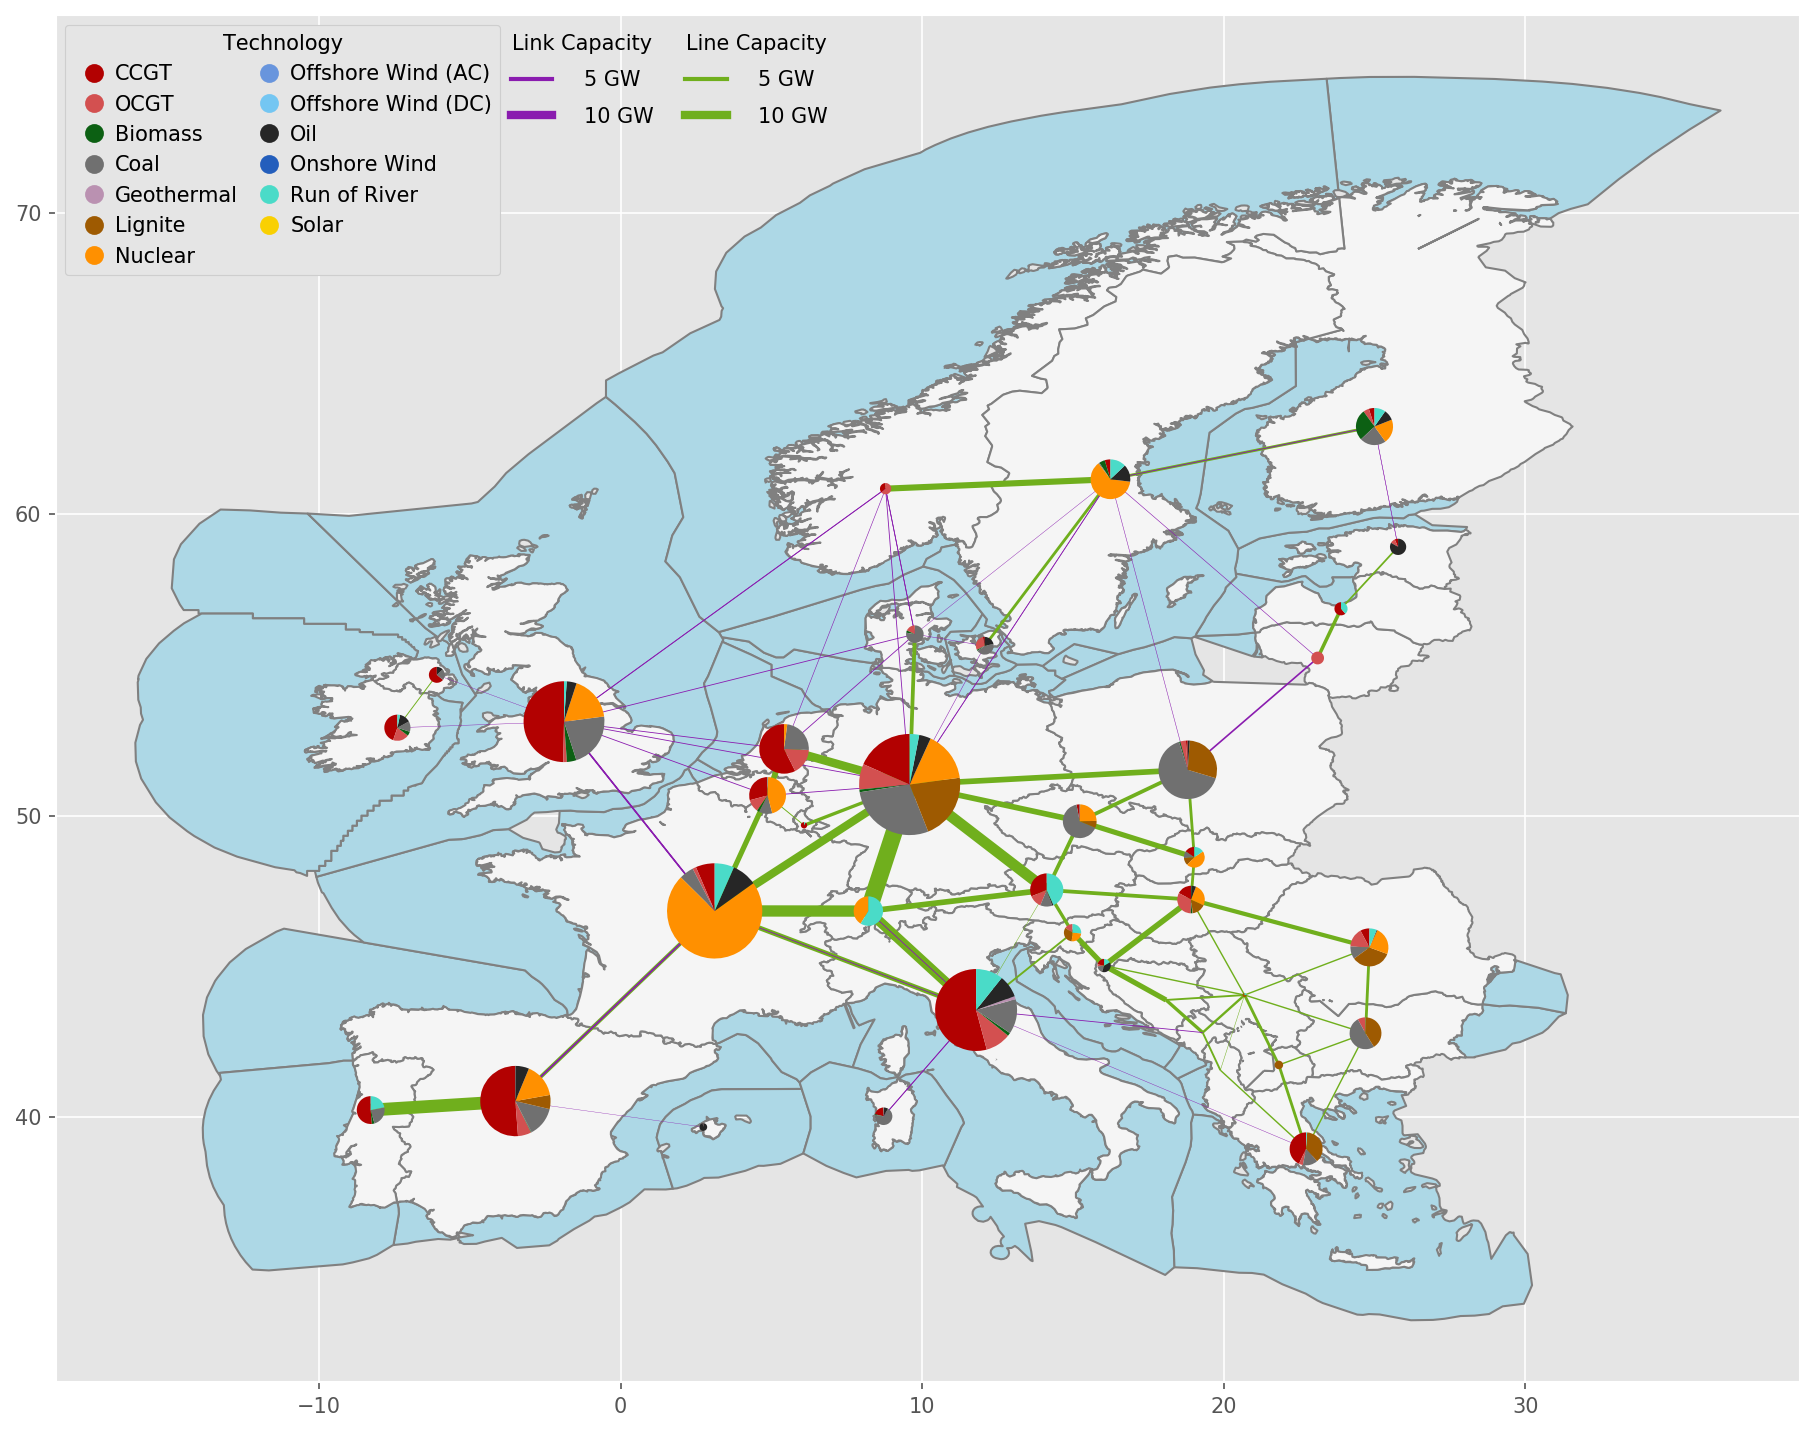
\includegraphics[width=7.5cm]{images/elec_s_37.png}

  {\footnotesize 
  PyPSA-Eur network clustered to 37 zones
  }
  \end{column}

  \begin{column}{8cm}
  {\small 
  \begin{itemize}
  \item In each scenario, we model the full European power system 
  clustered to \alert{37 zones}. 
    
  \item Each zone represents an individual country. Some countries are split to individual bidding zones, 
  such as DK1 (West) and DK2 (East).

  \item Consumers following 24/7 approach can be located in either of the \alert{four zones}: 
  Ireland, Denmark (zone DK1), Germany and the Netherlands.
    
  \item We assume that all consumers committed to 24/7 matching, form an alliance and sign contracts 
  with CFE generators so that their aggregated consumption can be matched 
  on an hour-by-hour basis with clean generation to achieve a given CFE matching score.
  
  \end{itemize}
  }
  
  \end{column}
  \end{columns}

\end{frame}



\begin{frame}{Scenario setup 2/3}

  {\small 
  \begin{itemize}

  \item We model various procurement policies and targets. The scenarios include: \\
  (i) \alert{24/7 CFE matching} with seven different CFE scores in a range from 80\% to 100\%, \\
  (ii) \alert{100\% annual matching} -- the best case scenario for the annual matching policy, \\
  (iii) \alert{A benchmark case} when 24/7 consumers cover theur load purely with grid purchases 
  without any policy regarding the origin of electricity.

  \item We conduct an analysis for different rates of participation. The two scenarios 
  assume that \alert{10\%} and \alert{25\%} of commercial and industrial load
  in a given zone participate in 24/7 CFE matching.

  \item We focus on two periods: \alert{2025} and \alert{2030}. The two periods differ by \\ 
  (i) Technology cost assumptions, \\
  (ii) National renewable expansion pathways,\\
  (iii) Power plant fleet (changes take place due to decomissioning based on generators' 
  age or national policies), \\
  (iv) System-wide assumptions, such as price for EU ETS allowances.

  \end{itemize}
  }
\end{frame}



\begin{frame}{Scenario setup 3/3}

  {\small 
  \begin{itemize}

  \item We assume that 24/7 consumers have an access to a wide palette
  of carbon-free technologies that are either available on the European market now
  or expected to be available for a commercial scale up in a close future. 
  
  \item We deliberately encode prospective technologies into the analysis.
  The \alert{technology inclusivity} is another 
  \hrefc{https://www.gstatic.com/gumdrop/sustainability/24x7-carbon-free-energy-methodologies-metrics.pdf}{important principle} 
  of the 24/7 CFE methodology. Thus, we consider carbon-free power generation
  technologies, which we believe can play important roles in facilitating CFE matching on hourly basis, 
  while enabling deeper decarbonization of electricity systems at the same time. 
  
  \item We formulate three scenarios grouping generators by a degree of technological
  maturity as of now \\
    \alert{Palette 1}: onshore wind, utility-scale solar, battery storage \\
    \alert{Palette 2}: all above + long-duration energy storage (hydrogen storage system) \\
    \alert{Palette 3}: all above + Allam Cycle natural gas generator + 
    advanced clean dispatchable generator (e.g., advanced geothermal system or advanced nuclear technology)

  \end{itemize}
  }
\end{frame}



%----------------------------------------
%----------------------------------------
\section{Data sources and key assumptions}


\begin{frame}{Summary of data sources: electricity grid}
 
  \begin{columns}[T]
  \begin{column}{7cm}

  \vspace{0.3cm}
  \centering

  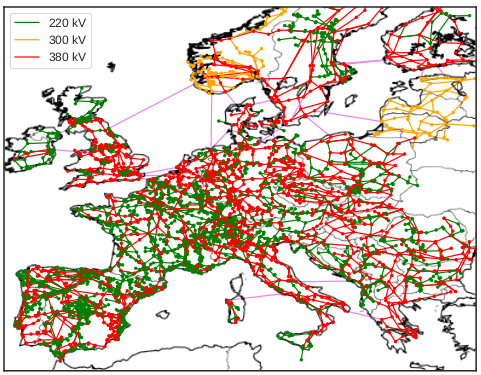
\includegraphics[width=7cm]{images/pypsa-eur-grid.png}

  {\footnotesize 
  \vspace{.1cm}
  Basic validation of grid model in 
  \hrefc{https://doi.org/10.1016/j.esr.2018.08.012}{Hörsch et al. (2018)}
  }
  \end{column}

  \begin{column}{7.5cm}
  {\small 
  \vspace{.3cm}
  \begin{itemize}
    \item Grid data contains AC lines at and above 220~kV voltage level, 
    all high voltage DC lines, and substations for the full 
    \hrefc{https://www.entsoe.eu/data/map/}{ENTSO-E area}.
    \item Grid data is collected by \hrefc{https://github.com/PyPSA/GridKit}{GridKit extraction} 
    of ENTSO-E interactive map
    \item Spatial resolution is
    \hrefc{https://pypsa-eur.readthedocs.io/en/latest/simplification/cluster_network.html}{adjustable}, 
    what allows spatial and topological analysis at different levels 
    (e.g. by transforming the transmission grid to a 380~kV only equivalent network).

  \end{itemize}
  }
  
  \end{column}
  \end{columns}

\end{frame}



\begin{frame}{Summary of data sources: power plants and technology costs}
 
  \begin{columns}[T]\

  \begin{column}{7.5cm}
    {\small 
    \begin{itemize}
      \item Existing generation fleet data is collected by cleaning, 
      standardizing and merging multiple power plant databases.
      
      \item The process is transparent and open-sourced via the 
      \hrefc{https://github.com/PyPSA/powerplantmatching}{powerplantmatching} package.
      The package provides all the important information about power plants in a ready-to-use format
      for the European power system. 
  
      \item Assumptions on energy system technologies (such as capital and operational costs, efficiencies, lifetimes, etc.) 
      are gathered from variety of open sources. The process is also open-sourced via the 
      \hrefc{https://github.com/PyPSA/technology-data}{technology-data} project. 
  
      \item Both tools are maintained by TU Berlin team.
  
    \end{itemize}
    }  
  \end{column}

  \begin{column}{7cm}

  \vspace{0.3cm}
  \centering

  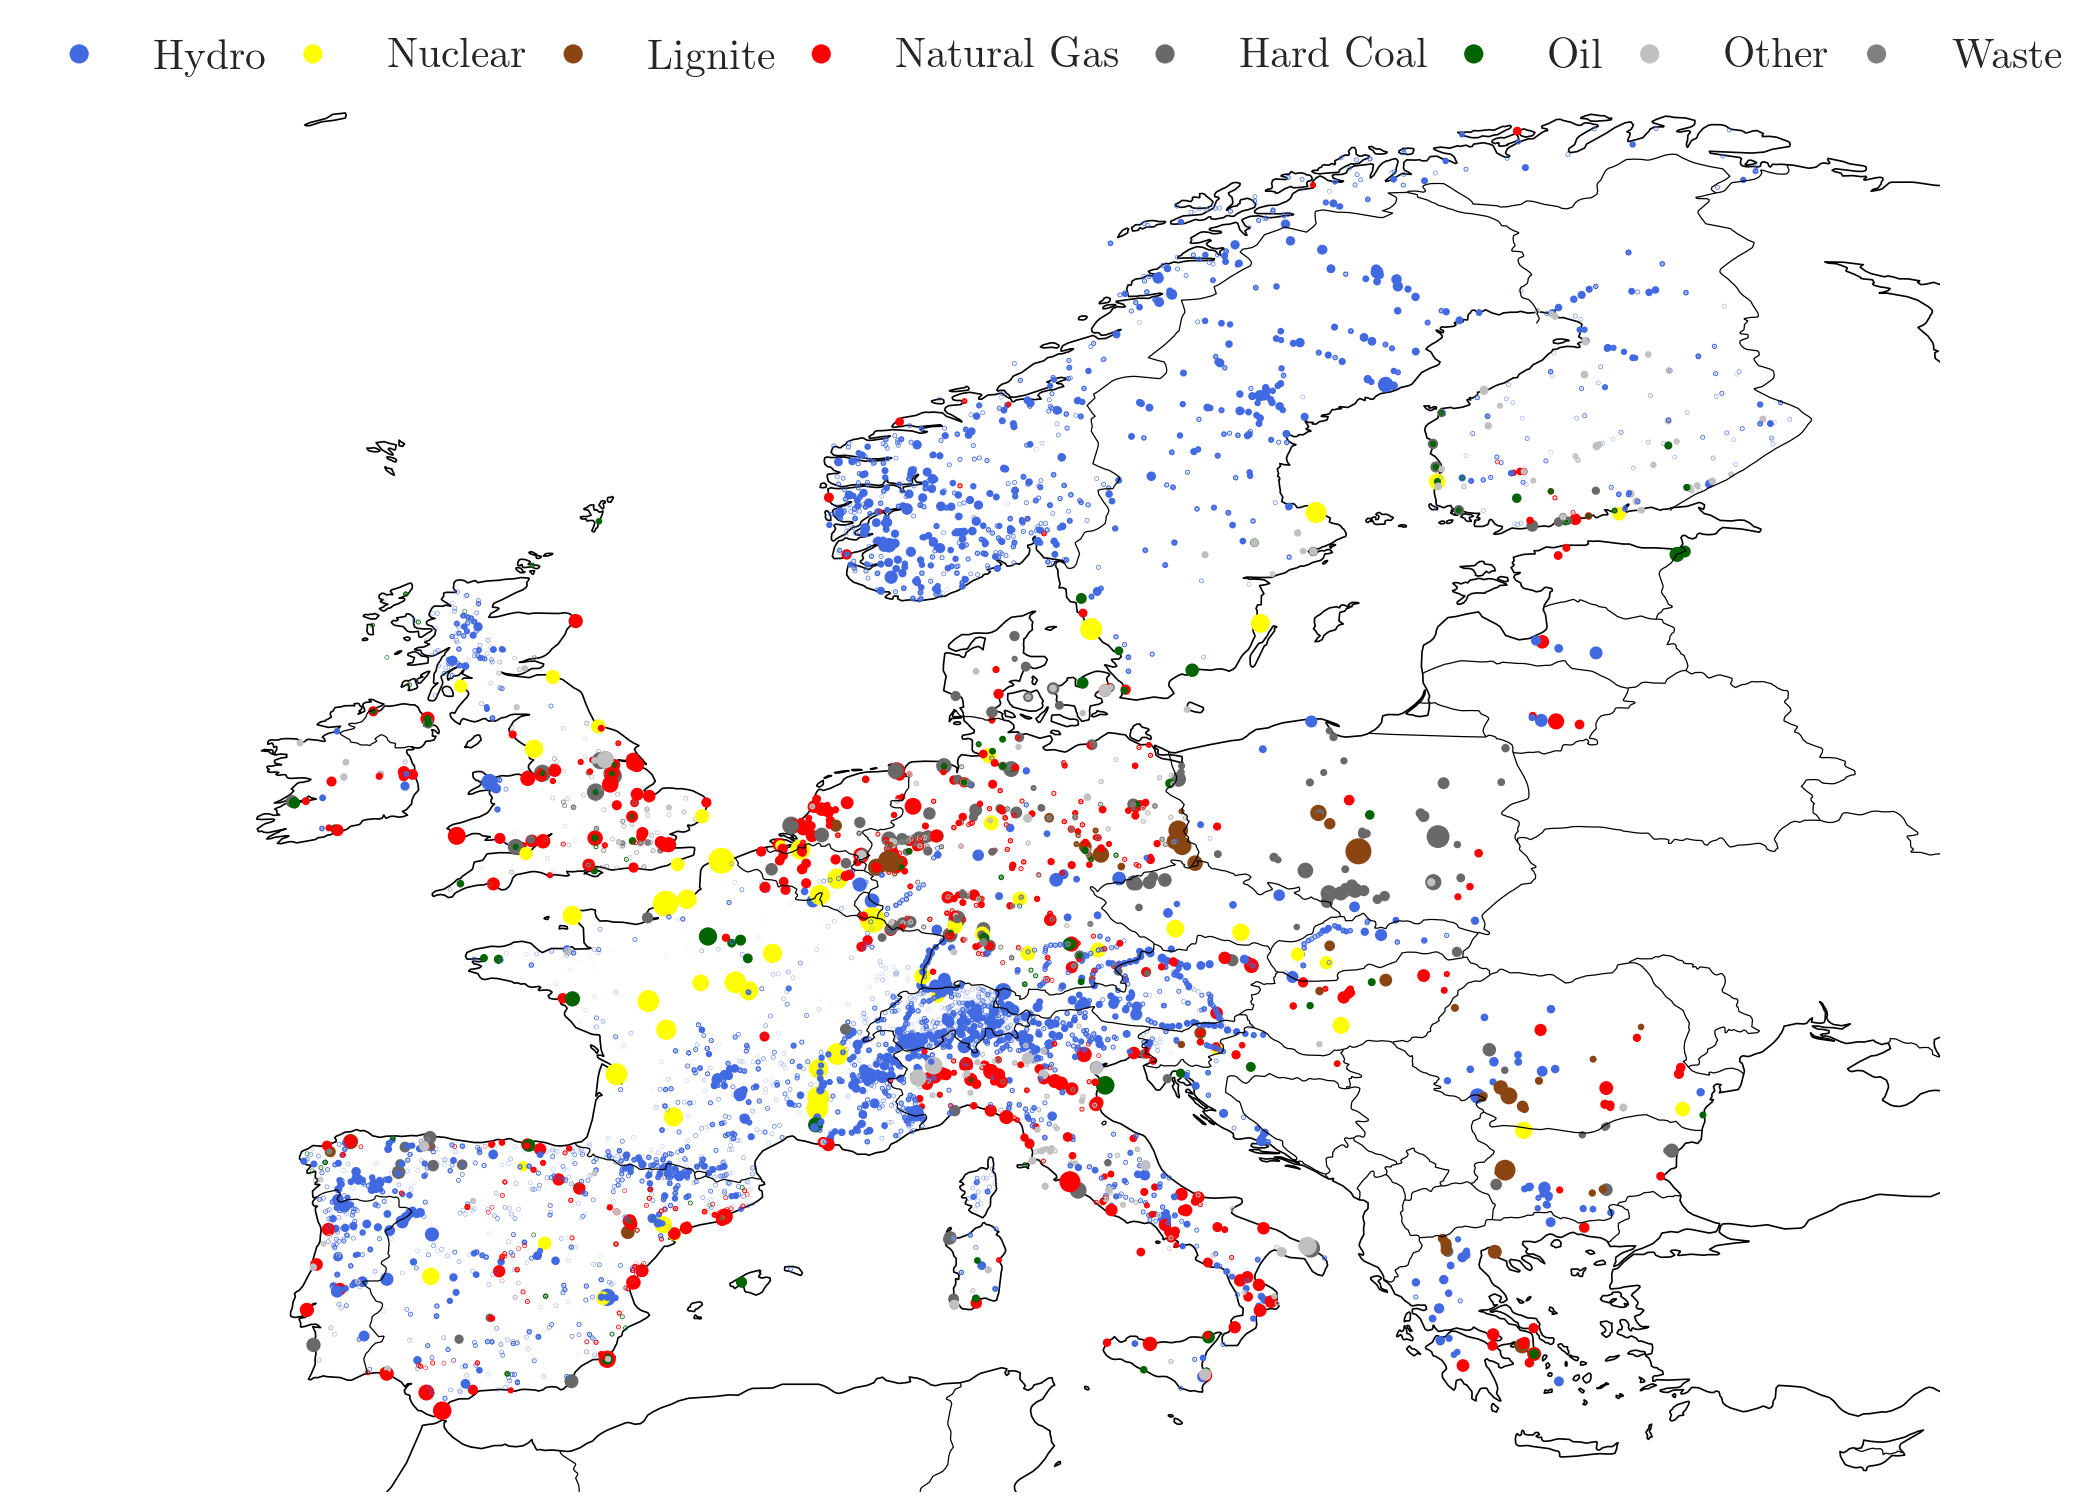
\includegraphics[width=7cm]{images/powerplantmatching.png}

  {\footnotesize 
  \vspace{0.1cm}
  A showcase example 
  of \hrefc{https://github.com/PyPSA/powerplantmatching}{powerplantmatching}
  }
  \end{column}
  \end{columns}

\end{frame}



\begin{frame}{Summary of data sources: renewable potentials and time series}
 
  \begin{columns}[T]
  \begin{column}{9cm}

  \vspace{0.3cm}
  \centering

  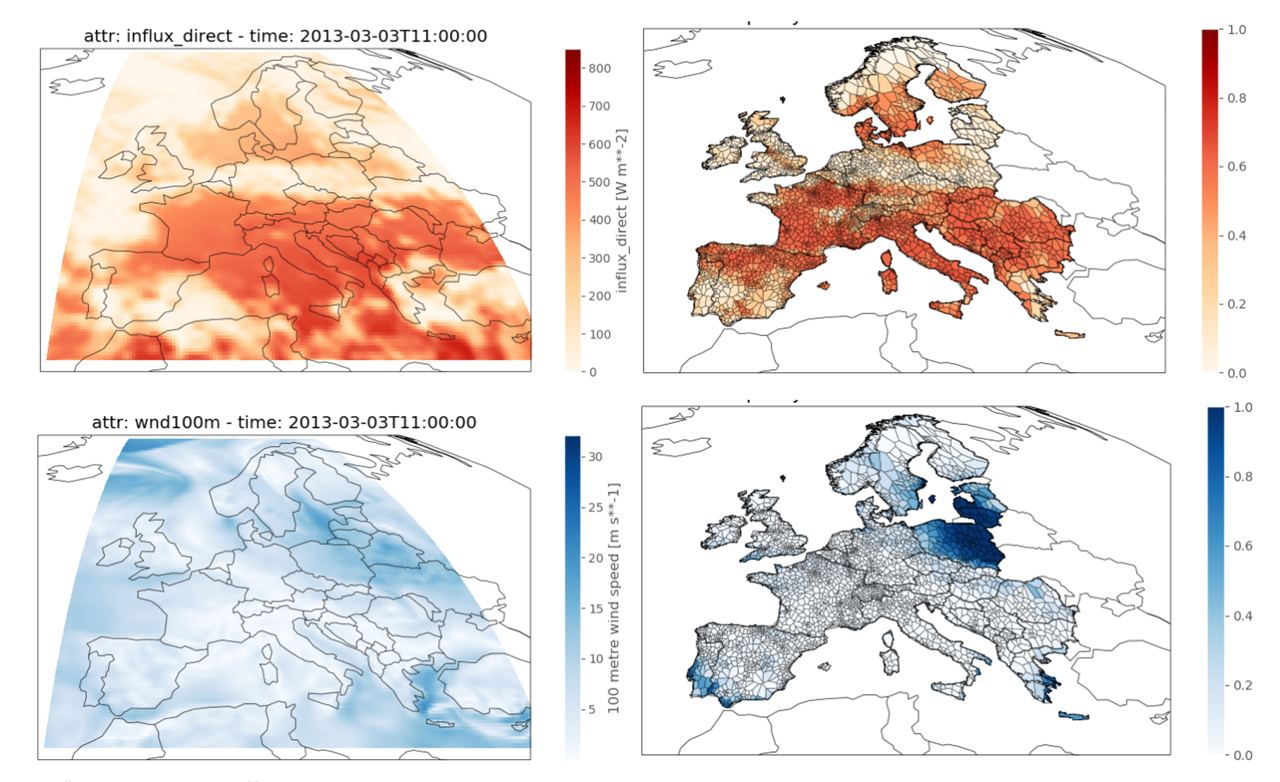
\includegraphics[width=9cm]{images/atlite.jpg}

  {\footnotesize 
  Converting weather data to energy system data with \hrefc{https://github.com/PyPSA/atlite}{atlite}
  }
  \end{column}

  \begin{column}{7cm}
  {\small 
  \begin{itemize}
    \item Renewable power potentials and generation profiles are processed by 
    the open-source \hrefc{https://github.com/PyPSA/atlite}{atlite} package, 
    which converts terabytes of weather data (like wind speeds, solar influx) 
    into the data for energy systems modelling.
    \item Geographic potentials for renewable energy are based on the
    \hrefc{https://github.com/FZJ-IEK3-VSA/glaes}{GLAES} framework. We gather and process
    datasets for land cover (CORINE2018), natural protection areas (NATURA2000),
    bathymetry (GEBCO2018) and \hrefc{https://pypsa-eur.readthedocs.io/en/latest/}{other} 
    to conduct own geospatial land availability analysis.
    \item The \alert{atlite} project is also maintained by TU Berlin team.

  \end{itemize}
  }
  
  \end{column}
  \end{columns}

\end{frame}


\begin{frame}{Other assumptions}

\begin{itemize}
  {\small 
\item Model is set to perform a \alert{single period}, \alert{perfect-foresight} optimization of investment 
and power dispatch decisions to meet electricity demand of the 24/7 consumers, 
as well as the demand of other consumers in the European electricity system for 2025 or 2030.
\item Electrical demand time-series is based on the 
\hrefc{https://open-power-system-data.org/}{OPSD project}. 
We assume the same demand profile per bidding zone for 2025 and 2030, as in the representative year 2013.
\item Similarly, we assume 2013 as the representative climate year for renewable in-feed.
\item Renewable expansion in the regional grid where 24/7 consumers are located is based on the 
\hrefc{https://energy.ec.europa.eu/topics/energy-strategy/national-energy-and-climate-plans-necps_en}{national energy and climate plans}.\footnote{{\scriptsize For Germany, we assume the 
\hrefc{https://www.bmwk.de/Redaktion/EN/Pressemitteilungen/2022/04/20220406-federal-minister-robert-habeck-says-easter-package-is-accelerator-for-renewable-energy.html}{Easter package}
to come into force as planned, i.e. RES cover 80\% of gross electricity consumption by 2030.}}
\item  National policies and decommissioning plans for coal and nuclear 
power plants are based on the 
\hrefc{https://beyond-coal.eu/}{Europe Beyond Coal}, 
and \hrefc{https://world-nuclear.org/}{world-nuclear.org} projects.
\item We assume price for EU ETS allowances to be 80~\euro/tCO$_2$ 
and 130~\euro/tCO$_2$ for 2025 and 2030, accordingly. The price for 
natural gas is assumed to be 35~\euro/MWh.\footnote{{\scriptsize Based on the price assumptions in the \hrefc{https://energy.ec.europa.eu/system/files/2022-05/SWD_2022_230_1_EN_autre_document_travail_service_part1_v3.pdf}{REPowerEU Plan}
issued by the European Commission in May 2022}}
}
\vspace{0.2cm}
\end{itemize}

\end{frame}


\begin{frame}{Technologies available for 24/7 consumers - 2025}
  
  {\scriptsize 

    \begin{tabular}{cccccccc}
      \hline
      Palette & Technology & CAPEX & FOM & VOM & Eff. & lifetime & Original reference \\
       &  & (overnight cost)  &  (\%/year) &  (€/MWh) & (per unit) & (years) & (\hrefc{https://github.com/PyPSA/technology-data}{technology data}) \\
      \hline
      1,2,3 & solar & 612 €/kW & 1.7 & 0.01 & - & 37.5 & \hrefc{https://ens.dk/en/our-services/projections-and-models/technology-data}{DEA}\\
      \hline
      1,2,3 & onshore wind & 1077 €/kW & 1.2 & 1.42 & - & 28.5 & \hrefc{https://ens.dk/en/our-services/projections-and-models/technology-data}{DEA}\\
      \hline
      1,2,3 & battery storage & 187 €/kWh & - & - & - & 22.5 & \hrefc{https://ens.dk/en/our-services/projections-and-models/technology-data}{DEA} \\
      \hline
      1,2,3  & battery inverter & 215 €/kW & 0.3 & - & 0.96  & 10.0 & \hrefc{https://ens.dk/en/our-services/projections-and-models/technology-data}{DEA} \\
      \hline
      2,3 & hydrogen storage\footnote{{\scriptsize Underground hydrogen storage in salt cavern}} 
                  & 2.5 €/kWh & 0 & 0 & - & 100.0 & \hrefc{https://ens.dk/en/our-services/projections-and-models/technology-data}{DEA} \\
      \hline
      2,3 & electrolysis & 550 €/kW & 2.0 & - & 0.67 & 27.5 & \hrefc{https://ens.dk/en/our-services/projections-and-models/technology-data}{DEA} \\
      \hline
      2,3 & fuel cell & 1200 €/kW & 5.0 & - & 0.50 & 10.0 & \hrefc{https://ens.dk/en/our-services/projections-and-models/technology-data}{DEA} \\
      \hline
      3 & NG Allam cycle\footnote{{\scriptsize Costs also include estimate of 40~€/ton for CO$_2$ transport \& sequestration.}} & 2760 €/kW & 14.8  & 3.2 & 0.54 & 30.0 &
      \hrefc{https://file.go.gov.sg/carbon-capture-utilisation-and-storage-decarbonisation-pathway-for-singapore-energy-and-chemical-sectors-pdf.pdf}{Navigant}, 
      \hrefc{https://netzeroamerica.princeton.edu/}{NZA}\\
      \hline
      3 & Advanced dispatchable\footnote{{\scriptsize A stand-in for clean dispatchable technologies, 
      such as advanced geothermal (closed-loop) systems. See e.g., \hrefc{https://www.eavor.com/}{Eavor} 
      developing a promising solution for clean baseload \& dispatchable power with a potential
      for a commercial scale up in Europe.}} 
      & 10000 €/kW & 0 & 0 & 1.00 & 30.0 & own estimates \\
      \end{tabular}
  }

\end{frame}



\begin{frame}{Technologies available for 24/7 consumers - 2030}
  
  {\scriptsize 

    \begin{tabular}{cccccccc}
      \hline
      Palette & Technology & CAPEX & FOM & VOM & Eff. & lifetime & Original reference \\
       &  & (overnight cost)  &  (\%/year) &  (€/MWh) & (per unit) & (years) & (\hrefc{https://github.com/PyPSA/technology-data}{technology data}) \\
      \hline
      1,2,3 & solar & 492 €/kW & 2.0 & 0.01 & - & 40 & \hrefc{https://ens.dk/en/our-services/projections-and-models/technology-data}{DEA}\\
      \hline
      1,2,3 & onshore wind & 1035 €/kW & 1.2 & 1.35 & - & 30 & \hrefc{https://ens.dk/en/our-services/projections-and-models/technology-data}{DEA}\\
      \hline
      1,2,3 & battery storage & 142 €/kWh & - & - & - & 25.0 & \hrefc{https://ens.dk/en/our-services/projections-and-models/technology-data}{DEA} \\
      \hline
      1,2,3  & battery inverter & 160 €/kW & 0.3 & - & 0.96  & 10.0 & \hrefc{https://ens.dk/en/our-services/projections-and-models/technology-data}{DEA} \\
      \hline
      2,3 & hydrogen storage\footnote{{\scriptsize Underground hydrogen storage in salt cavern}} 
                  & 2.0 €/kWh & 0 & 0 & - & 100 & \hrefc{https://ens.dk/en/our-services/projections-and-models/technology-data}{DEA} \\
      \hline
      2,3 & electrolysis & 450 €/kW & 2.0 & - & 0.68 & 30.0 & \hrefc{https://ens.dk/en/our-services/projections-and-models/technology-data}{DEA} \\
      \hline
      2,3 & fuel cell & 1100 €/kW & 5.0 & - & 0.5 & 10.0 & \hrefc{https://ens.dk/en/our-services/projections-and-models/technology-data}{DEA} \\
      \hline
      3 & NG Allam cycle\footnote{{\scriptsize Costs also include estimate of 40~€/ton for CO$_2$ transport \& sequestration.}}  & 2600 €/kW & 14.8  & 3.2 & 0.54 & 30 &
      \hrefc{https://file.go.gov.sg/carbon-capture-utilisation-and-storage-decarbonisation-pathway-for-singapore-energy-and-chemical-sectors-pdf.pdf}{Navigant}, 
      \hrefc{https://netzeroamerica.princeton.edu/}{NZA}\\
      \hline
      3& Advanced dispatchable\footnote{{\scriptsize A stand-in for clean dispatchable technologies, 
      such as advanced geothermal (closed-loop) systems. See e.g., \hrefc{https://www.eavor.com/}{Eavor} 
      developing a promising solution for clean baseload \& dispatchable power with a potential
      for a commercial scale up in Europe.}} 
      & 10000 €/kW & 0 & 0 & 1 & 30 & own estimates \\
      \end{tabular}
  }

\end{frame}


%---------------------------------------------
%---------------------------------------------
\section{Modelling results and analysis}


%----------------------------------------
\section{Conclusions and policy implications}


%----------------------------------------
\begin{frame}
  \frametitle{Open research and contacts}

  {\Large
  \alert{System-level impacts of 24/7 carbon-free electricity procurement in Europe}
  }

  \vspace{.3cm}
  All input data and code for this study is open and freely available at \\
  \hrefc{https://github.com/PyPSA/247-cfe}{https://github.com/PyPSA/247-cfe}

  \vspace{.3cm}
  For questions and inquiries related to this study, contact \\
  Dr. Iegor Riepin, iegor.riepin@tu-berlin.de \\
  Prof. Tom Brown, t.brown@tu-berlin.de

\end{frame}
\end{document}


%----------------------------------

\begin{frame}{Scenario: Participation 25\% - 2025 - IE - Palette 1 
\\ Fraction of demand met with carbon-free energy (CFE)}
\begin{columns}[T]
\begin{column}{9cm}
\centering

\includegraphics[width=9.9cm]{pr/25-2025-IE-p1-used.pdf}
\end{column}
\begin{column}{5cm}

  \begin{itemize}
  \item 100\% RES has only \alert{annual matching}
  \item 100\% RES PPA covers \alert{only 80\%} of hourly demand with CFE
  \item CFE target \alert{90\%} and beyond yields higher share of hourly demand met with CFE
  \item When CFE target approaches 100\%, C\&I participants rely \alert{only on procured resources}
  \end{itemize}
  
\end{column}
\end{columns}

\end{frame}



\begin{frame}{Scenario: Participation 25\% - 2025 - IE - Palette 1
\\ C\&I emission rate}

\begin{columns}[T]
\begin{column}{9cm}
\centering

\includegraphics[width=9.9cm]{pr/25-2025-IE-p1-ci_emisrate.pdf}
\end{column}
\begin{column}{5cm}

  \vspace{.5cm}

  \begin{itemize}
  \item CFE targets beyond \alert{85\%} yield lower emission rate than 100\% RES 
  \item As CFE target is tightened further, average emissions \alert{drop to zero}
  \end{itemize}
\end{column}
\end{columns}

\end{frame}



\begin{frame}{Scenario: Participation 25\% - 2025 - IE - Palette 1 \\
Cost breakdown with existing technologies (wind, solar, battery)}

\begin{columns}[T]
\begin{column}{9cm}
\centering

\includegraphics[width=9.9cm]{pr/25-2025-IE-p1-ci_costandrev.pdf}
\end{column}
\begin{column}{5cm}

  \vspace{.5cm}

  \begin{itemize}
  \item 100\% RES builds wind and solar
  \item Higher CFE targets \alert{include battery storage}
  \item 98\% CFE has \alert{cost premium of only 38\%} over 100\% RES
  \item Last 2\% more than \alert{doubles cost}
  \end{itemize}
\end{column}
\end{columns}

\end{frame}



\begin{frame}{Scenario: Participation 25\% - 2025 - IE - Palette 2 \\
Cost breakdown with long duration energy storage (LDES)}

\begin{columns}[T]
\begin{column}{9cm}
\centering

\includegraphics[width=9.9cm]{pr/25-2025-IE-p2-ci_costandrev.pdf}
\end{column}
\begin{column}{5cm}

  \vspace{.5cm}

  \begin{itemize}
  \item LDES (here 2.5 €/kWh hydrogen storage in caverns), significantly \alert{limits PPA cost increase}
  \item Cost premium of 98\% CFE is reduced to \alert{20\%} above 100\% RES
  \item 100\% CFE is \alert{only 34\%} above 100\% RES
  \end{itemize}
\end{column}
\end{columns}

\end{frame}


\begin{frame}{Scenario: Participation 25\% - 2025 - IE - Palette 3 \\
Cost breakdown with advanced dispatchable generators}

\begin{columns}[T]
\begin{column}{9cm}
\centering

\includegraphics[width=9.9cm]{pr/25-2025-IE-p3-ci_costandrev.pdf}
\end{column}
\begin{column}{5cm}


  \begin{itemize}
  \item Advanced geothermal could \alert{further limit cost}
  \item Firm generation could \alert{remove CFE cost premium}
  \item Results very \alert{sensitive} to cost assumptions (here overnight cost for AGS is at $10.000$~€/kW)
  \item NB Inclusion of clean firm generation reduces storage requirements and limits excess energy
  \item 
  \end{itemize}
\end{column}
\end{columns}

\end{frame}



\begin{frame}{Scenario: Participation 25\% - 2025 - IE - Palette 1 \\
System emissions (full ENTSO-E area),  1/2}

\begin{columns}[T]
\begin{column}{9cm}
\centering

\includegraphics[width=9.9cm]{pr/25-2025-IE-p1-system_emissions.pdf}
\end{column}
\begin{column}{5cm}

  \begin{itemize}
   \item  Here 550~MW of C\&I load in Ireland follows different procurement strategies
   \item 100\% RES can deliver greater system-level CO2 emissions reductions than lower CFE scores
   \item \alert{System emissions reduce} with higher CFE scores, as system-friendly CFE eats into fossil backup in system

  \end{itemize}
\end{column}
\end{columns}

\end{frame}


\begin{frame}{Scenario: Participation 25\% - 2025 - IE - Palette 1 \\
System-level emissions (full ENTSO-E area), 2/2}

\begin{columns}[T]
\begin{column}{9cm}
\centering

\includegraphics[width=9.9cm]{pr/25-2025-IE-p1-system_emissions.pdf}
\end{column}
\begin{column}{5cm}

  \begin{itemize}
   \item  Here 550~MW of C\&I load in Ireland follows different procurement strategies
   \item 100\% RES can deliver greater system-level CO2 emissions reductions than lower CFE scores
   \item \alert{Beyond 85\% CFE score}, 24/7 approach reduce system emissions to a greater extent than 100\% annual matching

  \end{itemize}
\end{column}
\end{columns}

\end{frame}

%----------------------------------------
%now explore IE-2030

\begin{frame}{The impacts of 2030 scenario  \\ 
Fraction of demand met with carbon-free energy (CFE) }

\begin{columns}[T]
\begin{column}{9cm}
\centering

\includegraphics[width=9.9cm]{pr/25-2025-IE-p1-used.pdf}
\end{column}
\begin{column}{5cm}

  \begin{itemize}
  \item Here results showed above for 25\%-\alert{2025}-IE-Palette~1
  \end{itemize}
  
\end{column}
\end{columns}

\end{frame}



\begin{frame}{The impacts of 2030 scenario \\ 
Fraction of demand met with carbon-free energy (CFE) }

\begin{columns}[T]
\begin{column}{9cm}
\centering

\includegraphics[width=9.9cm]{pr/25-2030-IE-p1-used.pdf}
\end{column}
\begin{column}{5cm}

  \begin{itemize}
  \item Here results showed above for 25\%-\alert{2025}-IE-Palette~1
  \item ... 25\%-\alert{2030}-IE-Palette~1
  \item 
  \end{itemize}
  
\end{column}
\end{columns}

\end{frame}


\begin{frame}{The impacts of 2030 scenario  \\ 
Fraction of demand met with carbon-free energy (CFE) }

\begin{columns}[T]
\begin{column}{9cm}
\centering

\includegraphics[width=9.9cm]{pr/25-2030-IE-p2-used.pdf}
\end{column}
\begin{column}{5cm}

  \begin{itemize}
  \item Here results showed above for 25\%-\alert{2025}-IE-Palette~1
  \item ... 25\%-\alert{2030}-IE-Palette~1
  \item ... 25\%-\alert{2030}-IE-Palette~2 (notice how LDES impacts 100\% CFE in 2030, which is not the case in 2025)
  \end{itemize}
  
\end{column}
\end{columns}

\end{frame}


\begin{frame}{The impacts of 2030 scenario  \\ 
Fraction of demand met with carbon-free energy (CFE) }

\begin{columns}[T]
\begin{column}{9cm}
\centering

\includegraphics[width=9.9cm]{pr/25-2030-IE-p3-used.pdf}
\end{column}
\begin{column}{5cm}

  \begin{itemize}
  \item Here results showed above for 25\%-\alert{2025}-IE-Palette~1
  \item ... 25\%-\alert{2030}-IE-Palette~1
  \item ... 25\%-\alert{2030}-IE-Palette~2 (notice how LDES impacts 100\% CFE in 2030, which is not the case in 2025)
 \item ... 25\%-\alert{2030}-IE-Palette~3 (with clean firm generation)
  \end{itemize}
  
\end{column}
\end{columns}

\end{frame}


\begin{frame}{The impacts of 2030 scenario\\
Intuitive effect on all metrics (selected: cost breakdown for Palette 2)}

\begin{columns}[T]
\begin{column}{9cm}
\centering

\includegraphics[width=9.9cm]{pr/25-2030-IE-p2-ci_costandrev.pdf}
\end{column}
\begin{column}{5cm}

  \begin{itemize}
  \item Electricity market developments from 2025 to 2030 (such as technology cost developments, national policies) \alert{decrease PPA cost}
  \item This also \alert{affects cost premium} of CFE vs 100\% annual matching 
  \item In this case, 100\% CFE cost decrease by 12\% compared to 2025 level, while 100\%~RES cost only by 5\%
 
  \end{itemize}
\end{column}
\end{columns}

\end{frame}

%----------------------------------------
%now jump to other countries for selected scenario branches 


\begin{frame}{The impacts of zone where C\&I participants are located}
\centering

Results for scenarios when C\&I load located in other zones show \alert{similar trends.} \\ 
However, each zone is has \alert{unique characteristics} that depend on local resources, national policies, interconnections, etc.

\end{frame}


%----------------------------------------

\begin{frame}{e.g. Germany (25\% - 2025 - DE - Palette~3) 
\\ Fraction of demand met with carbon-free energy (CFE)}

\begin{columns}[T]
\begin{column}{9cm}
\centering

\includegraphics[width=9.9cm]{pr/25-2025-DE-used.pdf}
\end{column}
\begin{column}{5cm}

  \begin{itemize}
  \item German grid is cleaner, in particular due to good interconnections with e.g., France and Denmark
  \item Similar trends to Irish results
  \end{itemize}
  
\end{column}
\end{columns}

\end{frame}

\begin{frame}{e.g. Germany (25\% - 2025 - DE - Palette~3) 
\\ C\&I emission rate}

\begin{columns}[T]
\begin{column}{9cm}
\centering

\includegraphics[width=9.9cm]{pr/25-2025-DE-ci_emisrate.pdf}
\end{column}
\begin{column}{5cm}

  \begin{itemize}
  \item German grid is cleaner, in particular due to good interconnections with e.g., France and Denmark
  \item Similar trends to Irish results
  \end{itemize}
  
\end{column}
\end{columns}

\end{frame}


\begin{frame}{e.g. Germany (25\% - 2025 - DE - Palette~3) 
\\ Cost breakdown with advanced dispatchable generators}

\begin{columns}[T]
\begin{column}{9cm}
\centering

\includegraphics[width=9.9cm]{pr/25-2025-DE-ci_costandrev.pdf}
\end{column}
\begin{column}{5cm}

  \begin{itemize}
  \item German grid is cleaner, in particular due to good interconnections with e.g., France and Denmark
  \item Similar trends to Irish results
  \end{itemize}
  
\end{column}
\end{columns}

\end{frame}


\begin{frame}{e.g. Germany (25\% - 2025 - DE - Palette~3) 
\\ Procured capacity by C\&I participants}

\begin{columns}[T]
\begin{column}{9cm}
\centering

\includegraphics[width=9.9cm]{pr/25-2025-DE-ci_capacity.pdf}
\end{column}
\begin{column}{5cm}

  \begin{itemize}
  \item  One of the unique features of German zone is it's size
  \item Here ca. \alert{9.6~GW} of C\&I load follows different procurement strategies
  \item This leads to relatively \alert{large amount of resources coming into system additionally} due to 24/7 procurement
  \end{itemize}
  
\end{column}
\end{columns}

\end{frame}



\begin{frame}{e.g. Germany (25\% - 2025 - DE - Palette~3) 
\\ Generation of resources procured by C\&I participants}

\begin{columns}[T]
\begin{column}{9cm}
\centering

\includegraphics[width=9.9cm]{pr/25-2025-DE-ci_generation.pdf}
\end{column}
\begin{column}{5cm}

  \begin{itemize}
  \item  One of the unique features of German zone is it's size
  \item Here ca. \alert{9.6~GW} of C\&I load follows different procurement strategies
  \item This leads to relatively \alert{large amount of resources coming into system additionally} due to 24/7 procurement
  \end{itemize}
  
\end{column}
\end{columns}

\end{frame}



\begin{frame}{e.g. Germany (25\% - 2025 - DE - Palette~3) 
\\ System-level capacity difference (rel. to reference scenario)}

\begin{columns}[T]
\begin{column}{9cm}
\centering

\includegraphics[width=9.9cm]{pr/25-2025-DE-total_capacity_diff.pdf}
\end{column}
\begin{column}{5cm}

  \begin{itemize}
  \item  Clean capacity procured by C\&I consumers displaces capacity built in the rest of the system 
  \item Here remarkable that \alert{C\&I clean resources substitute gas-fired technology}
  \item Inclusion of clean firm resources in C\&I portfolio \alert{helps to decarbonise} the entire electricity system
  \end{itemize}
  
\end{column}
\end{columns}

\end{frame}


%---------------------------------------------
%---------------------------------------------
\section{Additional scenarios}


\begin{frame}{The special scenario case}
\centering

Results for Denmark are pretty special. \\
This is driven by the Danish \hrefc{https://energy.ec.europa.eu/system/files/2020-01/dk_final_necp_main_en_0.pdf}{national energy and climate policy} \\ 
aimed at 110\% of renewable electricity in the consumption mix by 2030.

\end{frame}


\begin{frame}{Scenario: 25\% - 2030 - DK1 - Palette~2
\\ Fraction of demand met with carbon-free energy (CFE)}

\begin{columns}[T]
\begin{column}{9cm}
\centering

\includegraphics[width=9.9cm]{pr/25-2030-DK-p2-used.pdf}
\end{column}
\begin{column}{5cm}

\begin{itemize}
  \item Danish grid in 2030 is \alert{extremely clean}
  \item Only \alert{CFE scores above 95\%} deliver higher fraction of demand met with carbon-free energy than 100\% annual matching
\end{itemize}
  
\end{column}
\end{columns}

\end{frame}


\begin{frame}{Scenario: 25\% - 2030 - DK1 - Palette~2 \\ 
C\&I emission rate}

\begin{columns}[T]
\begin{column}{9cm}
\centering

\includegraphics[width=9.9cm]{pr/25-2030-DK-p2-ci_emisrate.pdf}
\end{column}
\begin{column}{5cm}

\begin{itemize}
  \item Danish grid in 2030 is \alert{extremely clean}
  \item Similar picture can be seen with the average emissions -- only \alert{CFE scores above 95\%} yield lower emission rate
  \item Even the reference case is at incredible 30~kg/MWh emission rate
\end{itemize}
  
\end{column}
\end{columns}

\end{frame}


\begin{frame}{Scenario: 25\% - 2030 - DK1 - Palette~2 \\ 
Cost breakdown with advanced dispatchable generators}

\begin{columns}[T]
\begin{column}{9cm}
\centering

\includegraphics[width=9.9cm]{pr/25-2030-DK-p2-ci_costandrev.pdf}
\end{column}
\begin{column}{5cm}

\begin{itemize}
  \item Danish grid in 2030 is \alert{extremely clean}
  \item The PPA cost is below 80~€/MWh level with just the LDES technology
\end{itemize}
  
\end{column}
\end{columns}

\end{frame}


%----------------------------------------
\section{Conclusions and policy implications}


\begin{frame}{Discussion:}

  \begin{itemize}
  \item 24/7 CFE procurement in Europe \alert{reduces emissions} both for buyer and for rest of system. The level of emission reduction is subject to zone where C\&I participants are located, as well as the time period.
  \item 75-90\% hourly CFE targets have \alert{only small cost premium} over annual RES matching.
  \item 100\% hourly CFE target \alert{comes at costs}. However, LDES can considerably decrease the cost premium. Inexpensive clean firm generation could nearly remove the cost premium.   
  \item 24/7 approach \alert{triggers investment in new technologies} the system will need later: long-duration storage and dispatchable clean generation.
  \item 24/7 approach \alert{benefits the rest of the system}, reducing emissions and flexibility needs.
  \end{itemize}

\end{frame}



\begin{frame}
  \frametitle{Open research and contacts}

  {\Large
  \alert{System-level impacts of 24/7 carbon-free electricity procurement in Europe}
  }

  \vspace{.3cm}
  All input data and code for this study is open and freely available at \\
  \hrefc{https://github.com/PyPSA/247-cfe}{https://github.com/PyPSA/247-cfe}

  \vspace{.3cm}
  For questions and inquiries related to this study, contact \\
  Dr. Iegor Riepin, iegor.riepin@tu-berlin.de \\
  Prof. Tom Brown, t.brown@tu-berlin.de

\end{frame}


%----------------------------------------
%----------------------------------------
\section*{Annex}


\end{document}